\documentclass[handout]{beamer}
\usetheme{Boadilla}
\usepackage{siunitx}
\usepackage[british]{babel}
\usepackage[backend=biber,sortcites,style=numeric,sorting=none,giveninits=true]{biblatex}
\usepackage{csquotes}
\usepackage{hyperref}
\addbibresource{bibliography.bib}

\graphicspath{{./figures/}}

\newcommand{\DimLength}{\mathsf{L}}
\newcommand{\DimTime}{\mathsf{T}}
\newcommand{\DimMass}{\mathsf{M}}
\newcommand{\DimCurrent}{\mathsf{I}}
\newcommand{\DimAmount}{\mathsf{N}}
\newcommand{\DimTemperature}{\Theta}
\newcommand{\DimLuminous}{\mathsf{J}}

\newcommand{\CarbonTwelve}{\textsuperscript{12}\textsf{C}}
\newcommand{\CarbonTwelveMath}{{}^{12}\mathsf{C}}
\newcommand{\AvogadroConstant}{N_{\text{A}}}
\newcommand{\BoltzmannConstant}{k_{\text{B}}}

\DeclareSIUnit{\atomicmassunit}{u}

\title{SI Units and Dimensions}
\author{Eason Shao}
\institute{St Paul's School}
\date{March 2025}

\AtBeginSection[]
{
    \begin{frame}
        \frametitle{Table of Contents}
        \tableofcontents[currentsection]
    \end{frame}
}

\begin{document}

\frame{\titlepage}

\frame{\tableofcontents}


\frame{
    \frametitle{Some Obsession \dots}

    \begin{itemize}
        \item I aim to typeset this slides properly, using the correct conventions as defined in the 2019 (9\textsuperscript{th}) SI Brochure \supercite{si-brochure} \dots \pause

        \item So the \textsf{siunitx} package is used. \pause

        \item In some places CIE Syllabus \supercite{cambridge-syllabus}/what we got taught slightly differs from the SI Brochure \supercite{si-brochure} \dots \pause

        \item And I will make it clear when they come up.
    \end{itemize}
}

\section{SI Units and their Correlation}

\frame{
    \frametitle{SI Base Units}

    There are 7 \emph{SI Base Units}, \pause each corresponding to a \emph{Dimension}.\pause

    \begin{table}
        \begin{tabular}{cccc}
            \hline
            \textbf{Quantity}         & \textbf{Name} & \textbf{Unit}        & \textbf{Dimension}         \\
            \hline\hline
            Time                      & second        & \(\unit{\second}\)   & \(\DimTime\)        \pause \\
            Length                    & metre         & \(\unit{\metre}\)    & \(\DimLength\)      \pause \\
            Mass                      & kilogram      & \(\unit{\kilogram}\) & \(\DimMass\)        \pause \\
            Electric Current          & ampere        & \(\unit{\ampere}\)   & \(\DimCurrent\)     \pause \\
            Amount of Substance       & mole          & \(\unit{\mole}\)     & \(\DimAmount\)      \pause \\
            Thermodynamic Temperature & kelvin        & \(\unit{\kelvin}\)   & \(\DimTemperature\) \pause \\
            Luminous Intensity        & candela       & \(\unit{\candela}\)  & \(\DimLuminous\)
        \end{tabular}

        \caption{SI Base Units}
        \label{tab:si-base}
    \end{table}
}

\frame{
    \frametitle{SI Derived Units}

    There are \emph{Derived Units}, represented as multiple of powers of the base units, perhaps with a numeric factor.\pause

    Those without are called \emph{Coherent Derived Units}. \supercite{wiki-si,si-brochure}\pause

    The list of Named SI Coherent Derived Units that we are required to know:

    \begin{table}
        \begin{tabular}{cccc}
            \hline
            \textbf{Quantity} & \textbf{Name}  & \textbf{Unit}                                                 & \textbf{Dimension}                              \\
            \hline\hline
            Plane Angle       & radian         & \(\qty{1}{\radian} = \qty{1}{\metre\per\metre}\)              & 1 \pause                                        \\
            Frequency         & hertz          & \(\qty{1}{\hertz} = \qty{1}{\second^{-1}}\)                   & \(\DimTime^{-1}\) \pause                        \\
            Activity          & becquerel      & \(\qty{1}{\becquerel} = \qty{1}{\second^{-1}}\)               & \(\DimTime^{-1}\) \pause                        \\
            Force             & newton         & \(\qty{1}{\newton} = \qty{1}{\kilogram\metre\per\second^2}\)  & \(\DimMass\DimLength\DimTime^{-2}\) \pause      \\
            Pressure          & pascal         & \(\qty{1}{\pascal} = \qty{1}{\newton\per\metre^2}\)           & \(\DimMass\DimLength^{-1}\DimTime^{-2}\) \pause \\
            Energy            & joule          & \(\qty{1}{\joule} = \qty{1}{\newton\metre}\)                  & \(\DimMass\DimLength^2\DimTime^{-2}\) \pause    \\
            Power             & watt           & \(\qty{1}{\watt} = \qty{1}{\joule\per\second}\)               & \(\DimMass\DimLength^2\DimTime^{-3}\) \pause    \\
            Celsius Temp.     & degree Celsius & \(t/\unit{\degreeCelsius} = T/\unit{\kelvin} - \num{273.15}\) & \(\DimTemperature\)
        \end{tabular}

        \caption{Some Named SI Coherent Derived Units}
        \label{tab:si-derived-1}
    \end{table}
}

\frame{
    \frametitle{And some more named coherent units \dots}

    \begin{table}
        \begin{tabular}{cccc}
            \hline
            \textbf{Quantity}       & \textbf{Name} & \textbf{Unit}                                     & \textbf{Dimension}                                             \\
            \hline\hline
            Electric Charge         & coulomb       & \(\qty{1}{\coulomb} = \qty{1}{\ampere\second}\)   & \(\DimCurrent\DimTime\) \pause                                 \\
            Electric P.D. (Voltage) & volt          & \(\qty{1}{\volt} = \qty{1}{\joule\per\coulomb}\)  & \(\DimMass\DimLength^2\DimTime^{-3}\DimCurrent^{-1}\) \pause   \\
            Capacitance             & farad         & \(\qty{1}{\farad} = \qty{1}{\coulomb\per\volt}\)  & \(\DimMass^{-1}\DimLength^{-2}\DimTime^4\DimCurrent^2\) \pause \\
            Electrical Resistance   & ohm           & \(\qty{1}{\ohm} = \qty{1}{\volt\per\ampere}\)     & \(\DimMass\DimLength^2\DimTime^{-3}\DimCurrent^{-2}\) \pause   \\
            Magnetic Flux           & weber         & \(\qty{1}{\weber} = \qty{1}{\volt\second}\)       & \(\DimMass\DimLength^2\DimTime^{-2}\DimCurrent^{-1}\) \pause   \\
            Magnetic Flux Density   & tesla         & \(\qty{1}{\tesla} = \qty{1}{\weber\per\metre^2}\) & \(\DimMass\DimTime^{-2}\DimCurrent^{-1}\)
        \end{tabular}

        \caption{Some More Named SI Coherent Derived Units}
        \label{tab:si-derived-2}
    \end{table}
}

\frame{
    \frametitle{Non-SI Units}

    There are some units that are not part of the SI system, but are still widely used in the scientific community.\pause

    The ones we should be aware of include:
    \begin{table}
        \begin{tabular}{cccc}
            \hline
            \textbf{Quantity} & \textbf{Name}    & \textbf{Unit}                                                              & \textbf{Dimension}                          \\
            \hline\hline
            Time              & minute           & \(\qty{1}{\minute} = \qty{60}{\second}\)                                   & \(\DimTime\)                                \\
            Time              & hour             & \(\qty{1}{\hour} = \qty{60}{\minute}\)                                     & \(\DimTime\)                                \\
            Time              & day              & \(\qty{1}{\day} = \qty{24}{\hour}\)                                        & \(\DimTime\) \pause                         \\
            Plane Angle       & degree           & \(\qty{1}{\degree} = \qty[parse-numbers=false]{\frac{\pi}{180}}{\radian}\) & 1 \pause                                    \\
            Energy            & electronvolt     & \(\qty{1}{\electronvolt} = \qty{1.60e-19}{\joule}\)                        & \(\DimMass\DimLength^2\DimTime^{-2}\)       \\
            Volume            & litre            & \(\qty{1}{\litre} = \qty{0.001}{\metre^3}\)                                & \(\DimLength^3\) \pause                     \\
            Mass              & tonne            & \(\qty{1}{\tonne} = \qty{1000}{\kilogram}\)                                & \(\DimMass\)                         \pause \\
            \hline
            Mass              & atomic mass unit & \(\qty{1}{\atomicmassunit} =  \qty{1.66e-27}{\kilogram}\)                  & \(\DimMass\)
        \end{tabular}

        \caption{Some non-SI units accepted for use with SI units}
        \label{tab:non-si}
    \end{table}
}

\frame{
    \frametitle{Dimension and Units}

    When I first learnt physics, my dad told me that we could only add/subtract quantities with the same units \dots \pause \space but we can actually add quantities with the same dimensions.\pause

    To actually find the value, we have to convert them to the same units, and adjust the values of the quantities.\pause

    \begin{itemize}
        \item A \emph{dimension} is a property of a physical quantity, and\pause
        \item A \emph{unit} is a standard for measuring that quantity.\pause
    \end{itemize}

    A unit incorporates the idea of a \emph{scale} to the value measured.\pause

    CIE: \textbf{All physical quantities consist of a numerical magnitude value and a unit.} \supercite{cambridge-syllabus}
}

\frame{
    \frametitle{Dimensional Analysis}

    \begin{itemize}
        \item CIE: \textit{Use SI base units to check the homogeneity of physical equations}. \supercite{cambridge-syllabus} \emph{Dimensional} analysis isn't exactly mentioned.\pause

        \item \emph{Note:} For a quantity \(Q\), The SI Brochure \supercite{si-brochure} uses \(\dim Q\) for the dimension of \(Q\), \([Q]\) for the unit of \(Q\), and \(\{Q\}\) for the numerical value of \(Q\). \(Q = \{Q\} [Q]\).\pause

        \item \emph{Dimensional Analysis} is checking the \emph{homogeneity} of an equation, by comparing the dimensions of the quantities on both sides of the equation.\pause

        \item Dimensional Analysis does not allow us to find the dimensionless constants involved, but it can help us find the form of the equation, and we can find the constant by some other means (e.g. experiment).
    \end{itemize}
}

\section{Definition of SI Units}

\frame{
    \frametitle{Overview}

    \begin{figure}
        \centering
        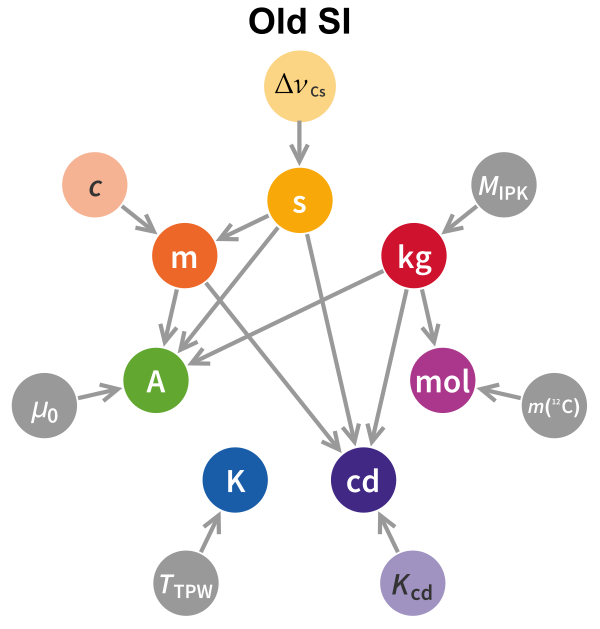
\includegraphics[width=0.4\textwidth]{new-si.svg.png}
        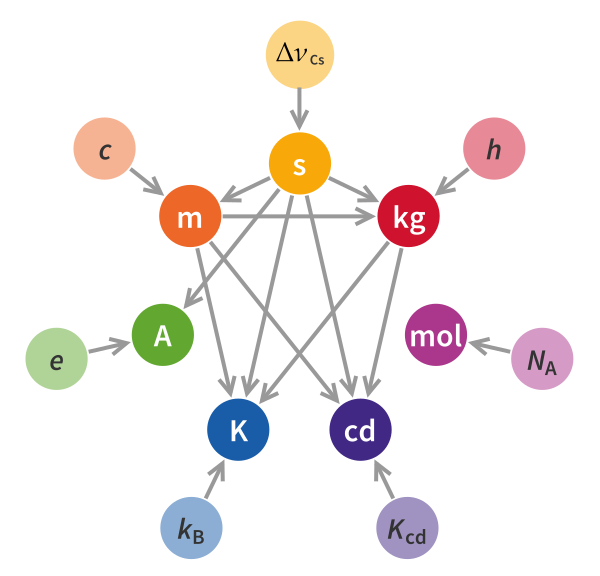
\includegraphics[width=0.4\textwidth]{old-si.svg.png}
        \caption{The Definitions of Units \supercite{si-diagram,wiki-redef}}
        \label{fig:si-units-definition}
    \end{figure}

    The second, the metre and the candela remained unchanged.
}

\frame{
    \frametitle{The Kilogram}

    The old SI relies on the \emph{International Prototype of the Kilogram} (IPK) as the standard for the kilogram. But \dots \pause

    \begin{figure}
        \centering
        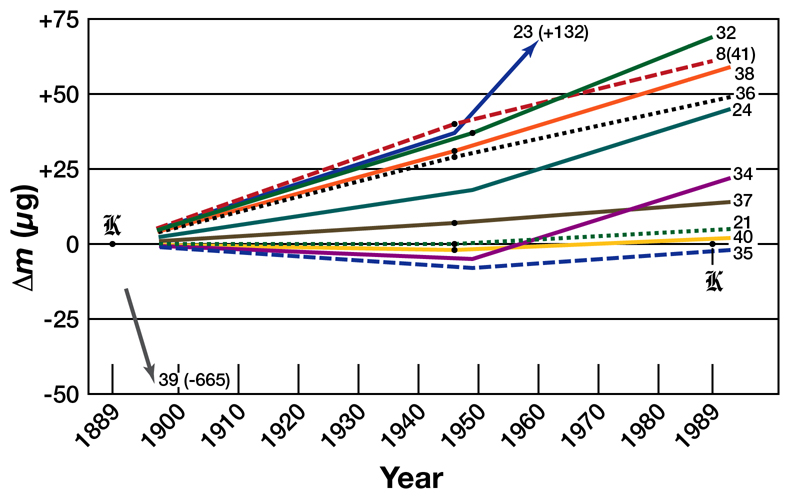
\includegraphics[width=0.75\textwidth]{mass-drifts.jpg}
        \caption{The Mass Drifts of the National Prototypes \supercite{periodic-verification, wiki-ipk}}
        \label{fig:international-prototype-kilogram}
    \end{figure}
}

\frame{
    \frametitle{The Kilogram}

    Considering that mass and \emph{energy} are equivalent, we can use some energy to define mass! (Since speed of light is exactly \(c = \qty{299792458}{\metre\per\second}\), and \(E = mc^2\).) \pause

    We already have the second and the metre defined. \pause

    So we could use the energy of a photon with a certain frequency! \(E = hf.\)\pause

    \[
        h = \qty{6.62607015e-34}{\joule\second}.
    \]
}

\frame{
    \frametitle{The Ampere}

    The old SI relies on the force between parallel conductors as the standard for the ampere: \supercite{wiki-redef}

    \[
        \mu_0 = \qty[parse-numbers=false]{4 \pi \times 10^{-7}}{\henry\per\metre}.
    \]\pause

    This relies on force, which has dimensions \(\DimMass\DimLength\DimTime^{-2}\).\pause

    Another constant that we could use is:
    \[
        e = \qty{1.602176634e-19}{\coulomb}.
    \]\pause

    So now the Ampere still depends on the second, but is no longer dependent on mass or length! \supercite{wiki-ampere}\pause

    \emph{Notice that how the ampere is defined in terms of the coulomb, but is still the base unit.}
}

\frame{
    \frametitle{The Kelvin}

    The old SI relies on the triple point of water as \(\qty{273.16}{\kelvin}\). (The zero is fixed by the nature of thermodynamics.)\pause

    \begin{figure}
        \centering
        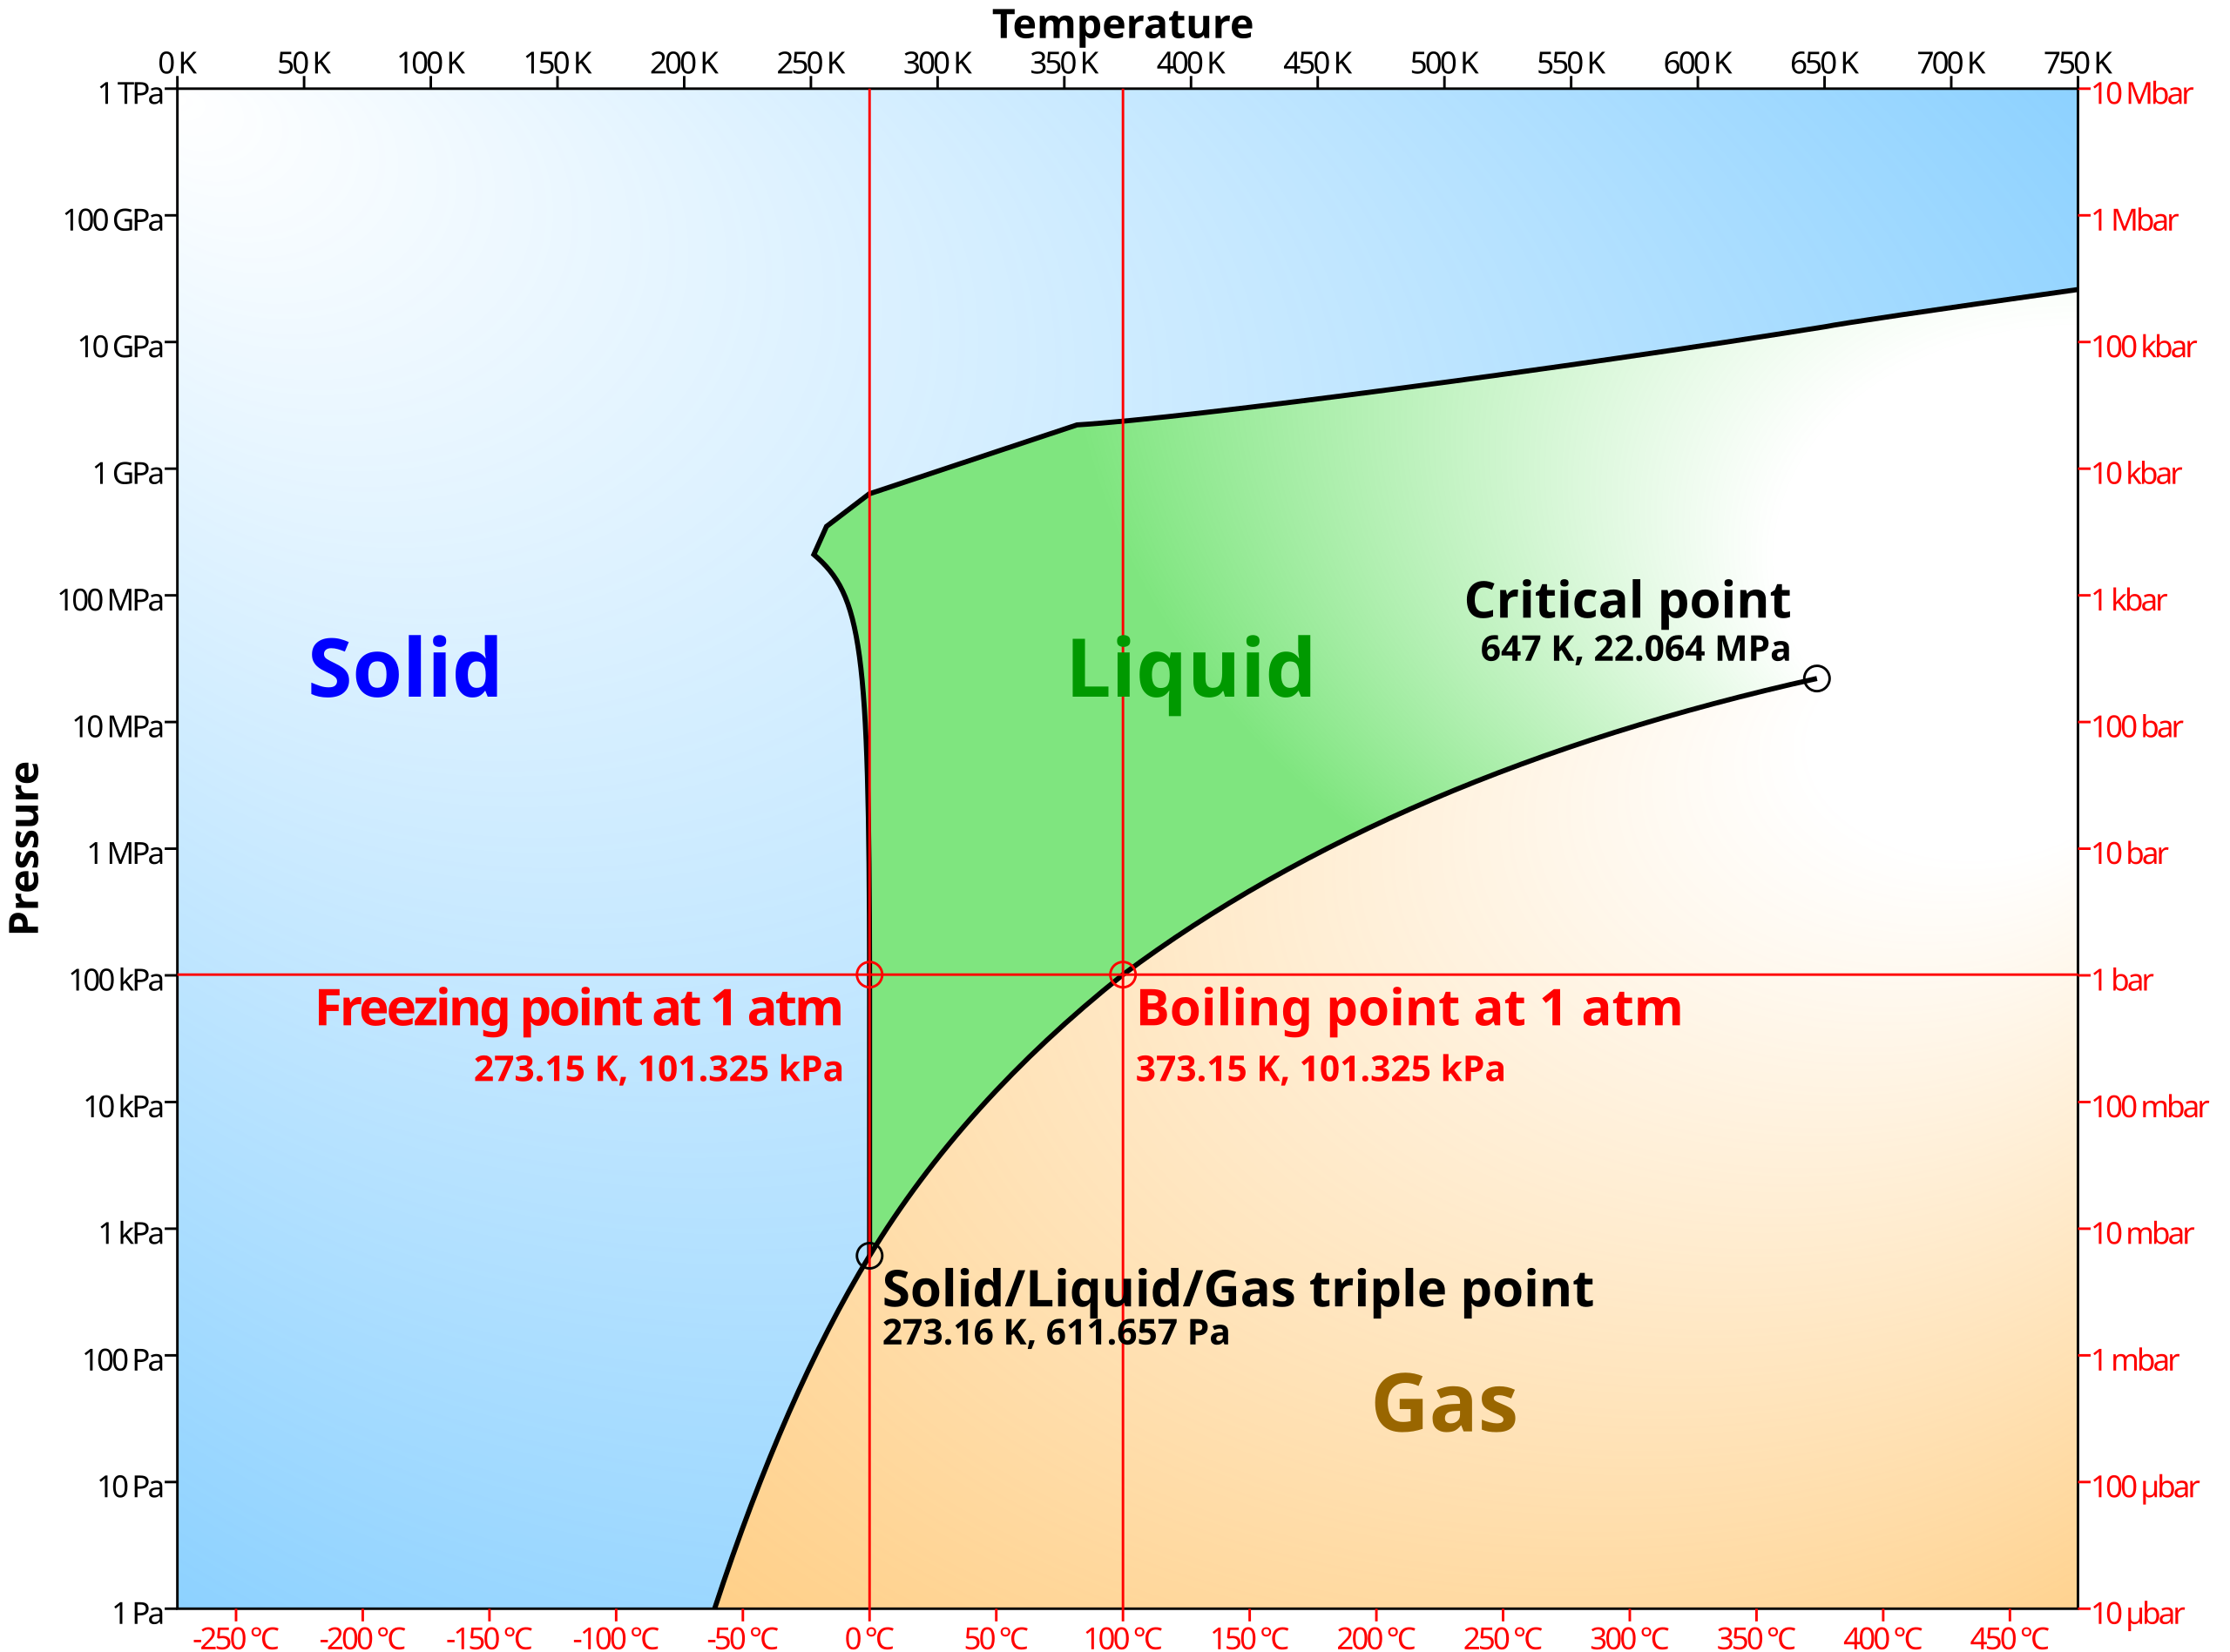
\includegraphics[width=0.4\textwidth]{phase-diagram-water.svg.png}
        \caption{The Phase Diagram of Water \supercite{water-diagram}}
        \label{fig:triple-point-water}
    \end{figure}

    To remove the need to accurately measure the triple point of water, they choose to let it depend on the Boltzmann constant \(\BoltzmannConstant\). \supercite{wiki-kelvin}
    \[
        \BoltzmannConstant = \qty{1.380649e-23}{\joule\per\kelvin}.
    \]
}

\frame{
    \frametitle{The Mole}

    This might be the most controversial unit, but it also brings the most controversial change in the SI Unit System. \pause

    Previously, the mole was defined as the number of atoms in \(\qty{12}{\gram}\) of \CarbonTwelve. \pause

    Similar to the kelvin, this relies on the measurement of some physical stuff (a sphere of atoms to be measured). So we chose to some constant, the Avogadro constant \(\AvogadroConstant\):
    \[
        \AvogadroConstant = \qty{6.02214076e23}{\per\mole}.
    \]\pause

    This brings a problem: one of these two has to be demolished: \supercite{wiki-redef}\pause
    \begin{itemize}
        \item The mass of a \CarbonTwelve \space atom is exactly \(\qty{12}{\dalton}\).\pause
        \item The number of dalton in a gram is exactly \(\AvogadroConstant\).
    \end{itemize}
}

\frame{
    \frametitle{The Mole}

    The SI Brochure chose to preserve the former and demolish the latter:\pause

    \begin{quote}
        The dalton (\(\unit{\dalton}\)) and the unified atomic mass unit (\(\unit{\atomicmassunit}\)) are alternative names (and symbols) for the same unit, equal to \(1/12\) of the mass of a free carbon 12 atom, at rest and in its ground state. \supercite{si-brochure}
    \end{quote}\pause

    This is just simply bad -- because the ratio of one gram to one dalton is no longer perfectly the Avogadro's constant \pause-- or is it?\pause

    \begin{quote}
        According to the present definition \(M(\CarbonTwelveMath)\) is no longer known exactly and must be determined experimentally. The value chosen for \(\AvogadroConstant\) is such that at the time of adopting the present definition of the mole, \(M(\CarbonTwelveMath)\) was equal to \(\qty{0.012}{\kilogram\per\mole}\) with a relative standard uncertainty of \(\num{4.5e-10}\). \supercite{si-brochure}
    \end{quote}
}

\frame{
    \frametitle{The Constants}

    \begin{align*}
        h                     & = \qty{6.62607015e-34}{\kilogram\metre\squared\per\second}                  \\
        e                     & = \qty{1.602176634e-19}{\ampere\second}                                     \\
        \BoltzmannConstant    & = \qty{1.380649e-23}{\kilogram\metre\squared\per\kelvin\per\second\squared} \\
        \AvogadroConstant     & = \qty{6.02214076e23}{\per\mole}                                            \\
        c                     & = \qty{299792458}{\metre\per\second}                                        \\
        \Delta\nu_{\text{Cs}} & = \qty{9192631770}{\per\second}                                             \\
        K_{\text{cd}}         & = \qty{683}{\candela\steradian\second\cubed\per\kilogram\per\metre\squared}
    \end{align*}
}

\frame{
    \frametitle{Why we need units, and the SI?}
    \begin{quote}
        Physics, and natural science in general, is a reasonable enterprise based on valid experimental evidence, criticism, and rational discussion. \supercite{experiment-in-physics}
    \end{quote}
}

\section*{Appendices}

\frame[allowframebreaks]{
    \frametitle{References}

    \printbibliography
}

\end{document}